
In this chapter, we evaluate our quantification model and inference algorithms on simulated datasets with constant expected degradation rates and real direct RNA-seq datasets with sequencing spike-ins. 

\section{Methods for benchmarking}

We benchmark our model against three existing methods for transcript quantification from long-read RNA-seq. 

\paragraph{bambu} Reference guided transcript discovery and quantification for long read RNA-seq data.
\paragraph{FLAIR} Full-Length Alternative Isoform analysis of RNA.
\paragraph{NanoCount} EM based transcript abundance from nanopore reads.

\section{Evaluations on simulated data}

To evaluate our model's ability to correct for degradation bias, we simulated five datasets for a range of degradation rates $\mathbb{E}[d]\in\{0.05,0.1,0.2,0.4,0.5\}$. In addition, we simulated reads for artificial novel isoforms that are modified by dropping exons from the 5' end of selected reference isoforms, termed \textit{subset} isoforms. This increases the proportion of multi-mapping reads and makes correcting for degradation bias crucial for accurate transcript quantification. See Appendices \ref{ap:gen-novl-iso} and \ref{ap:sim-deg-reads} for more details on novel isoform and degraded read simulation. 

\subsection{Comparisons between model variations}

\subsection{Comparisons with existing methods}

\begin{figure}[H]
    \centering
    \includegraphics[width=\textwidth]{figures/sec-4-scc-nrmse.png}
    \caption[Empirical results for SCC and NRMSE on simulated datasets]{Spearman correlation coefficient (SCC) and normalized root-mean-squared error (NRMSE) on simulated datasets with different degradation rates $\mathbb{E}[d]=\{0.05,0.1,0.2,0.4,0.5\}$. \textbf{a.} SCC across all simulated isoforms. \textbf{b.} SCC across subset isoforms. \textbf{c.} NRMSE across all simulated isoforms. \textbf{d.} NRMSE across all subset isoforms.}
    \label{fig:sec-4-scc-nrmse}
\end{figure}

\begin{figure}[H]
    \centering
    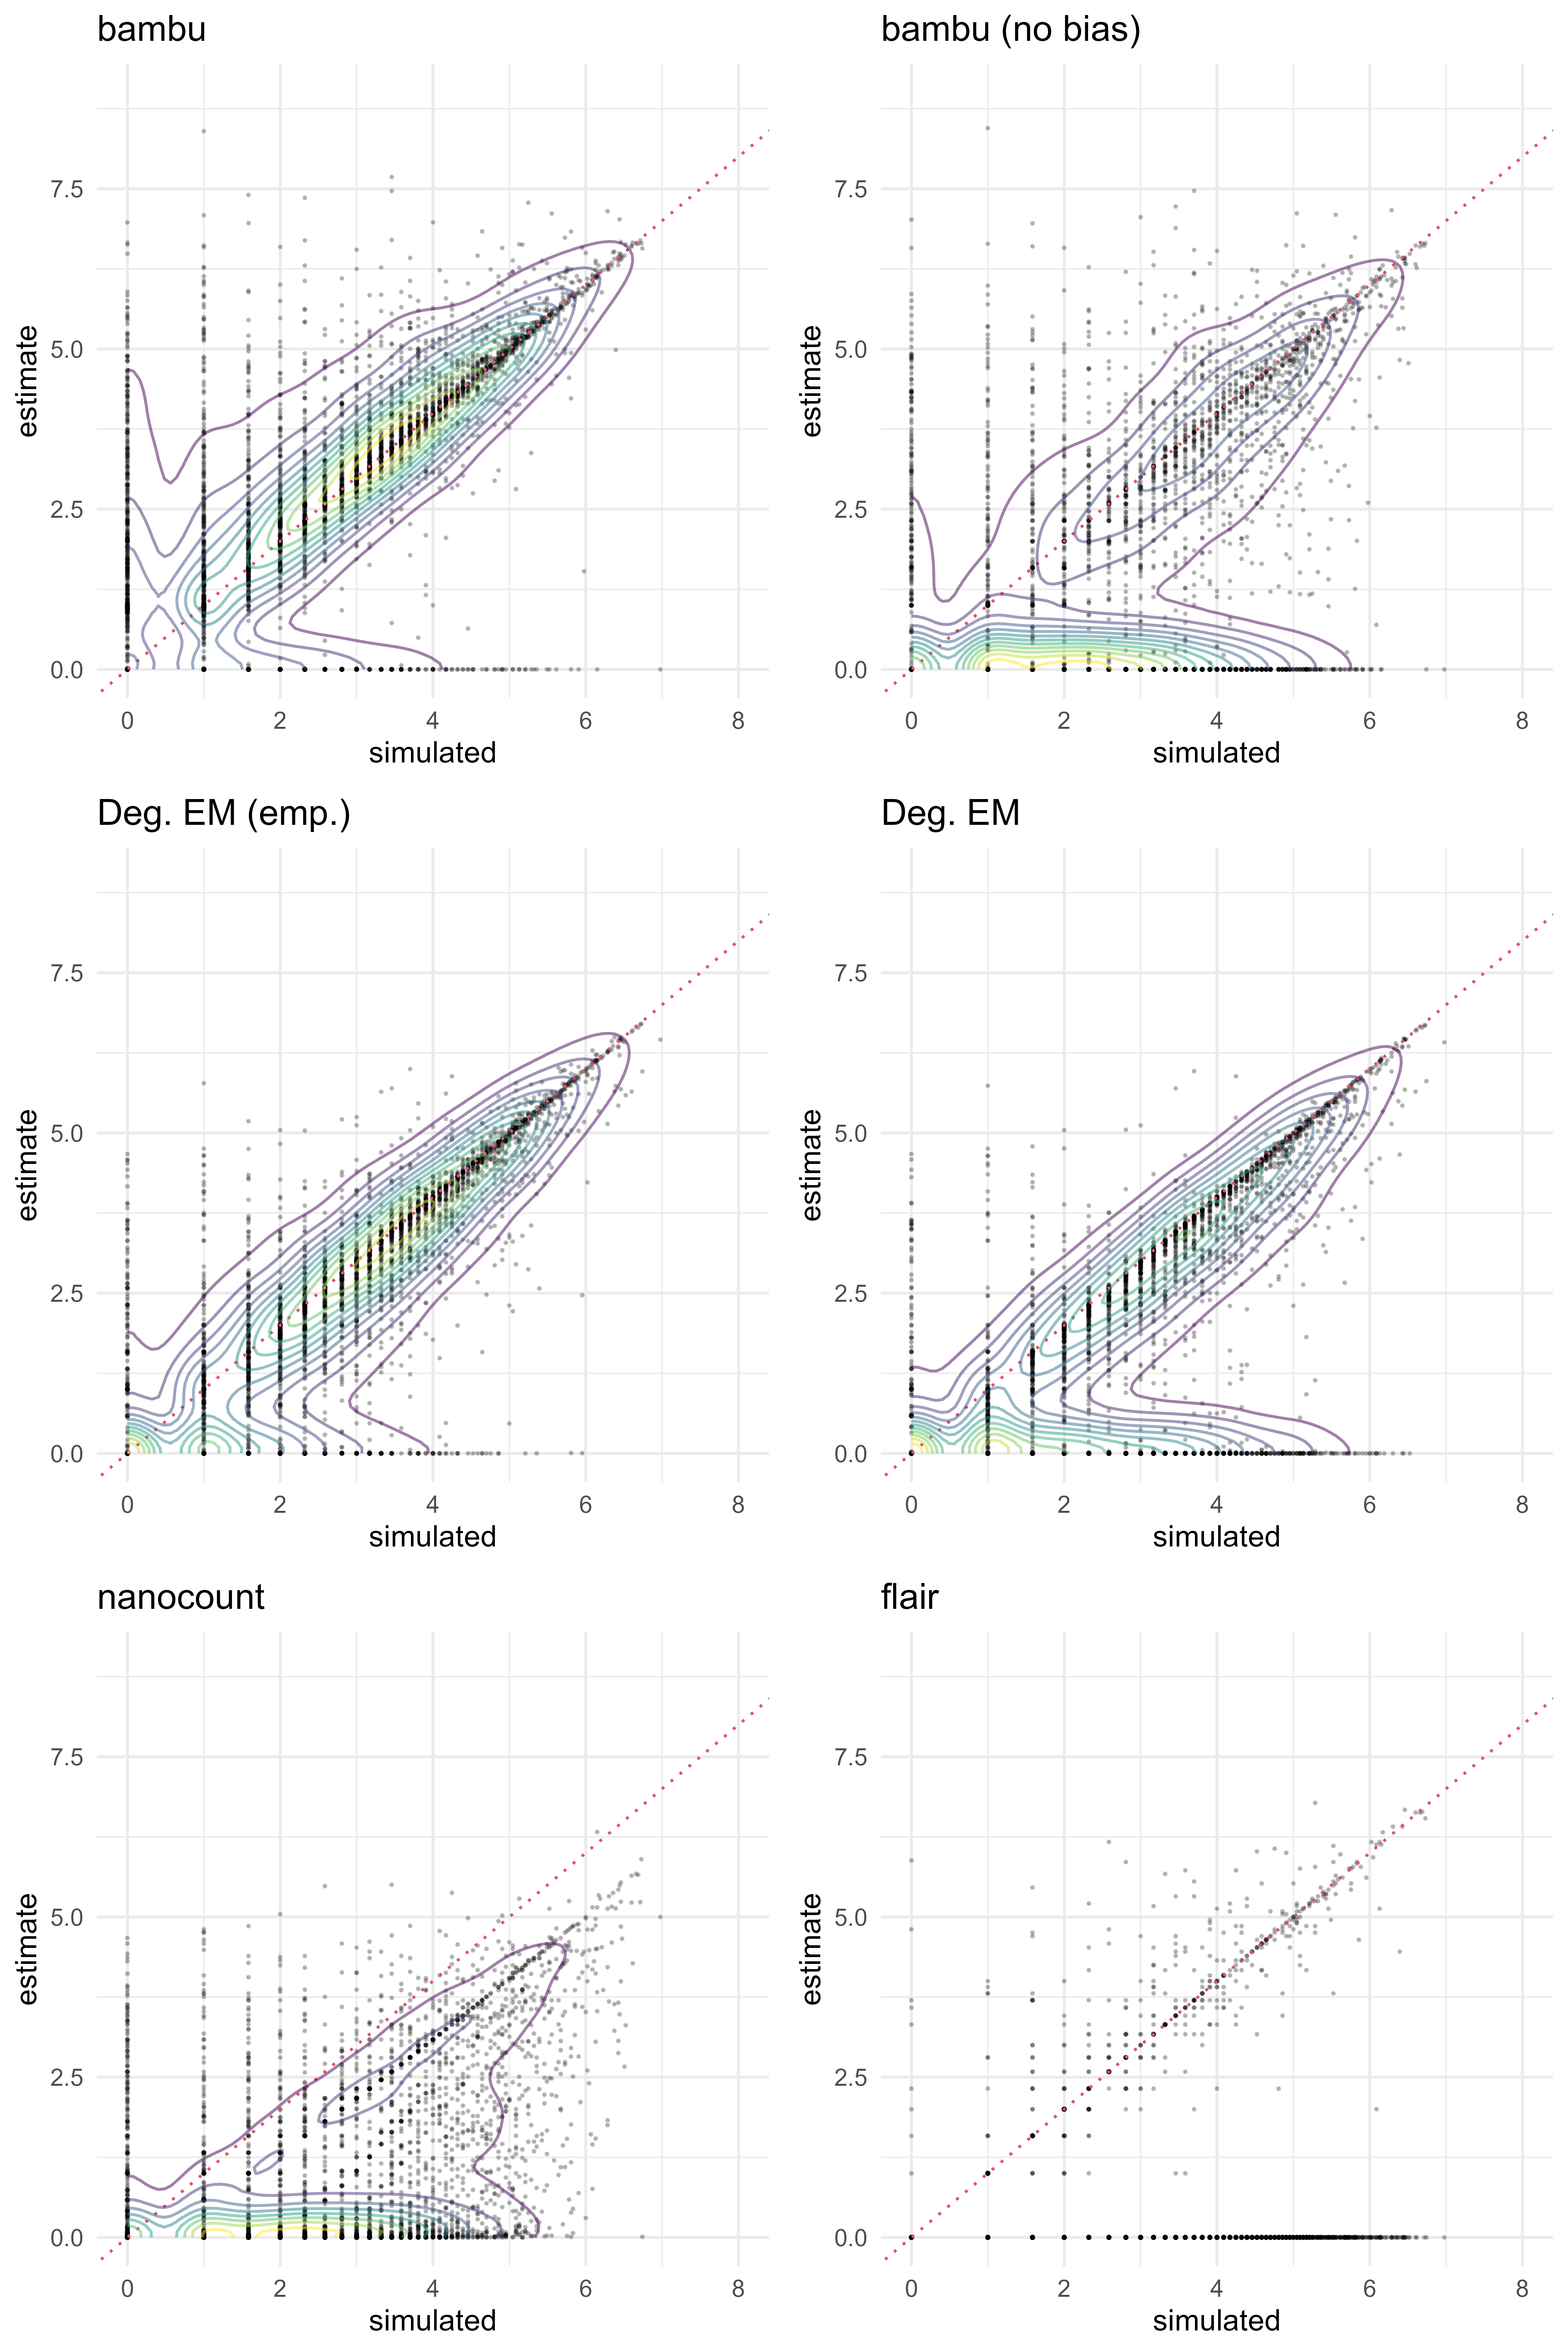
\includegraphics[width=0.9\textwidth]{figures/sec-4-scatter-hard.png}
    \caption[Scatter plots on subset isoforms in a simulated dataset with $\mathbb{E}d=0.2$]{Scatter plots on subset isoforms in a simulated dataset with $\mathbb{E}[d]=0.2$ across the methods. Counts are $\log_2$ transformed with the addition of 1 pseudocount. A kernel density (KDE) is fitted to show the density of points. No KDE is fitted for flair due to the abundance of zeroes. The diagonal is indicated by the dotted line.}
    \label{fig:sec-4-scatter-hard}
\end{figure}

\begin{table}[htbp]
  \centering
    \begin{tabular}{|l|P{2cm}|P{2cm}|P{2cm}|P{2cm}|}
\cline{2-5}    \multicolumn{1}{r|}{} & \multicolumn{2}{c|}{All isoforms} & \multicolumn{2}{c|}{Subset isoforms} \bigstrut\\
    \hline
    Method & SCC   & NRMSE & SCC   & NRMSE \bigstrut\\
    \hline
    bambu & 0.771 & 0.599 & 0.671 & 1.009 \bigstrut\\
    \hline
    bambu (no bias) & 0.74  & 0.636 & 0.432 & 1.165 \bigstrut\\
    \hline
    Deg. EM & 0.826 & 0.485 & 0.612 & 0.635 \bigstrut\\
    \hline
    Deg. EM (emp.) & \textbf{0.874} & \textbf{0.393} & \textbf{0.811} & \textbf{0.43} \bigstrut\\
    \hline
    flair & 0.697 & 0.696 & 0.153 & 1.176 \bigstrut\\
    \hline
    nanocount & 0.778 & 0.536 & 0.466 & 0.987 \bigstrut\\
    \hline
    \end{tabular}%
    \caption[Empirical results for mean SCC and NRMSE on simulated datasets]{Mean spearman correlation coefficient (SCC) and normalized root-mean-squared error (NRMSE) across simulated datasets with different degradation rates $\mathbb{E}[d]=\{0.05,0.1,0.2,0.4,0.5\}$. Bold values in each column represent the best result for the corresponding metric.}
  \label{tab:addlabel}%
\end{table}%

\begin{figure}[H]
    \centering
    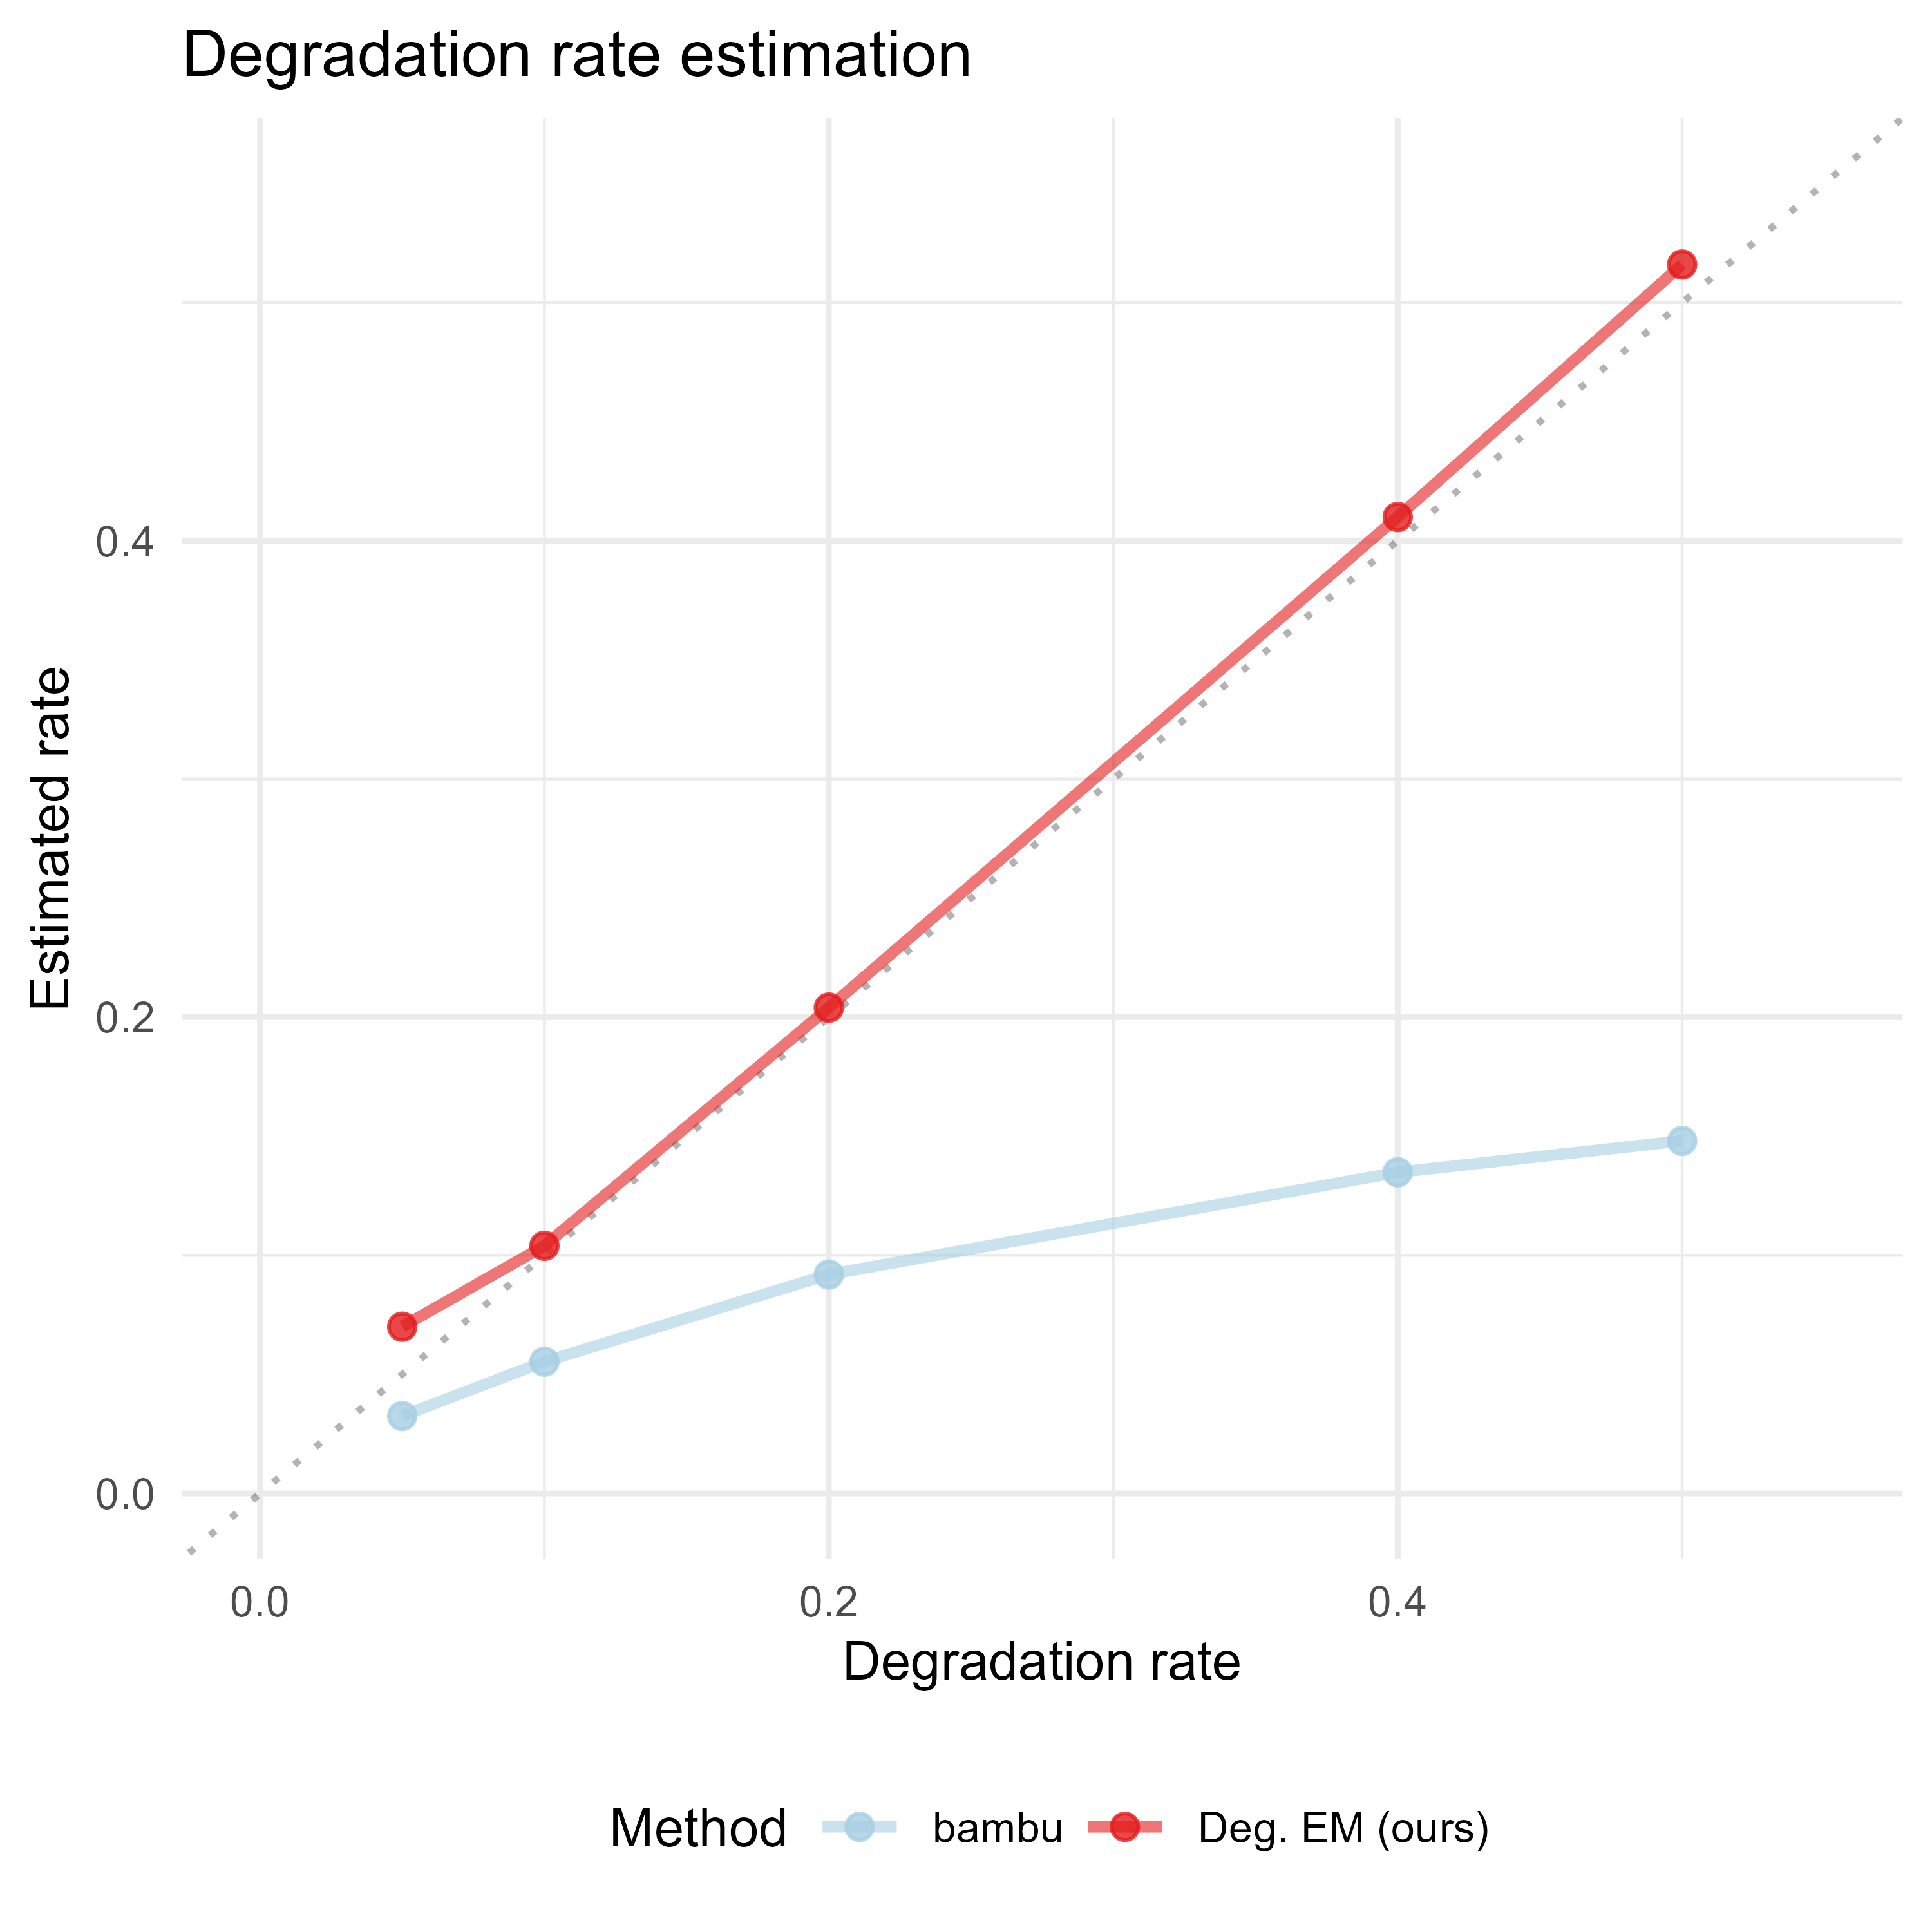
\includegraphics[width=0.7\textwidth]{figures/sec-4-deg-est.png}
    \caption[Empirical results for degradation rate estimation on simulated datasets]{Comparison of the degradation rates estimated by bambu and our model on simulated datasets with different degradation rates $\mathbb{E}[d]=\{0.05,0.1,0.2,0.4,0.5\}$. The diagonal is indicated by the dotted line.}
    \label{fig:sec-4-deg-est}
\end{figure}

\section{Evaluations on real data}

Six H9 samples (600ng mRNA + 1\% spike-in of 6ng SIRV-4) sequenced with direct RNA-seq.

\subsection{Comparisons with existing methods}